%!TEX root = ../../main.tex
\section{RSConverter}
RS485-bussen er valgt til at kommunikere på, se hvorfor i teknologiundersøgelsen. Til dette formål er udformet et simpelt kredsløb vha. MAX3082. Det logiske 0-5V UART-signal fra PSoC 4 konverteres til et differentielt signal, som kører ud på bussen, og vice versa.

\begin{figure}[H]
	\centering
	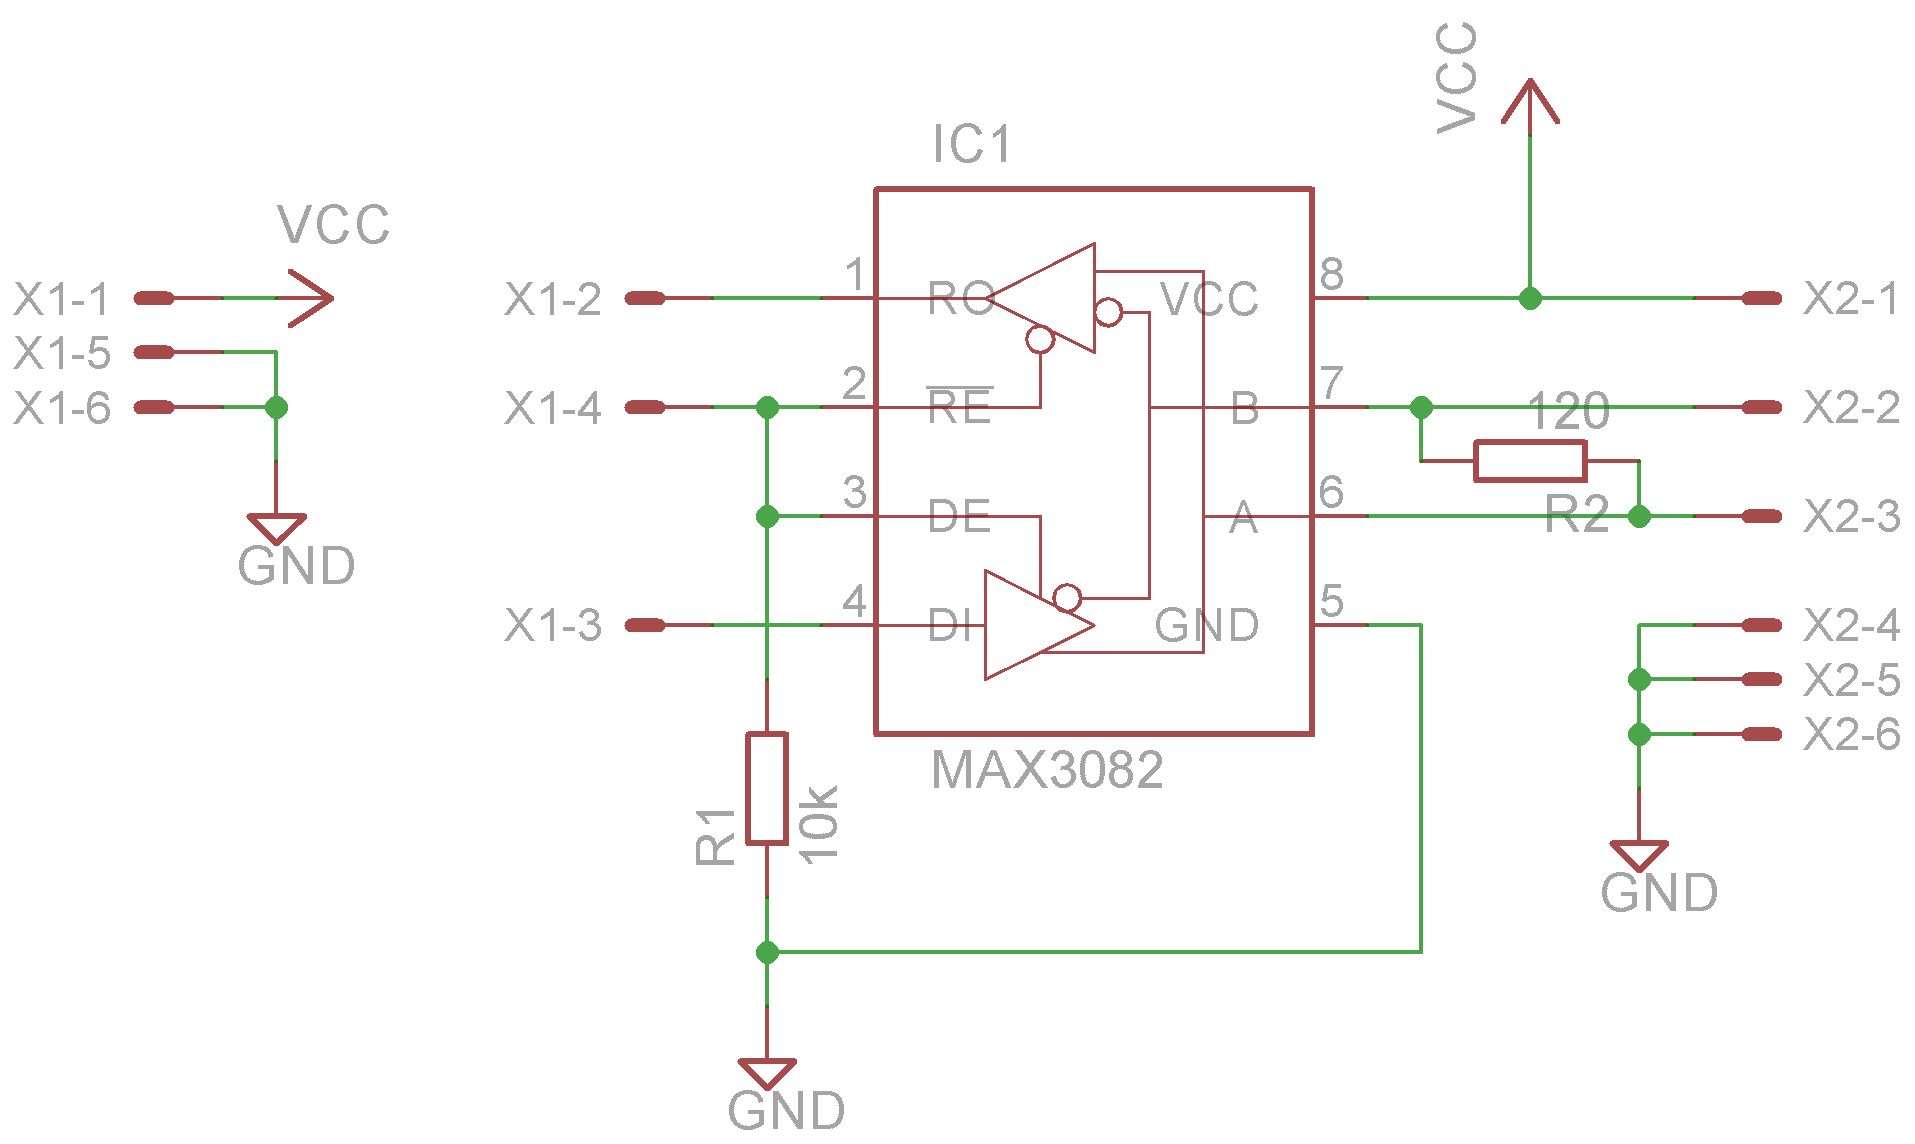
\includegraphics[scale=1]{../Hardware/RS485_Converter/Schematic}
	\caption{RS485 converter}
	\label{photo:RS485converter}
\end{figure}

$R_1$ er en pulldown-modstand der sørger for, at standard-tilstanden af kredsen står til at modtage. Når der sendes ud på bussen, kræver det en høj $Tx_{Enable}$. $R_2$ fungerer som terminering på bussen og sørger for at undgå reflektion af signalet. Størrelsen af modstanden afhænger derfor af tranmissionslinjen (bussen). Når $R_2 = R_{bus}$ bliver hele signalet overført. 
\\\\
Det er samtidigt vigtigt at bussen kun termineres i starten og enden. Dvs. hvis der er koblet flere kar på KarBussen, skal de serieforbindes og den sidste samt den første have en termineringsmodstand. I guiden for RS485 kommunikation anbefales det, at man bruger $120\ohm$ kabler og derfor termineres der med $120\ohm$. 
\\\\
For at udregne det maksimale strømforbrug til videre design af PSU kigges i databladet for MAX3082. Under "Absolute Maximum Ratings" findes det, at i et 8-pin plastic DIP hus som det der anvendes, har et maksimal effektforbrug på 727mW.

Udregningen af det maksimale strømforbrug bliver derfor følgende:
\begin{equation}
	I = \frac{P}{U} = \frac{727mW}{5V} = 145,4mA
\end{equation}

\fxnote{Scopebilleder, forklaringer osv.}